\documentclass{article}

\usepackage{graphicx}
\usepackage[margin=1in]{geometry}
\usepackage{booktabs}
\usepackage{float}
\usepackage{amsmath}
\usepackage[hidelinks]{hyperref}

\begin{document}

\title{Radial Kernel \texorpdfstring{$f_i$}{fi} Optimization Report}
\author{}
\date{27 February 2026}
\maketitle

\section*{Approach}
\subsection*{\hypertarget{ans1}{1. Radial \texorpdfstring{$f_i$}{fi} optimization method}}
The notebook parameterizes a 2D kernel using radial bins:
\[
K(x,y)=\sum_{r=0}^{R} f_r\,B_r(x,y),\quad R=10
\]
where $B_r$ are ring-shaped basis masks and $f_r$ are learnable radial coefficients.

\vspace{0.5em}
\textbf{Optimization objective:}
\[
\mathcal{L}=\mathcal{L}_{\text{BCE}}+\lambda_{\text{smooth}}\,\frac{1}{R}\sum_{r=1}^{R}(f_r-f_{r-1})^2+\lambda_{\text{anchor}}\,\frac{1}{R+1}\sum_{r=0}^{R}(f_r-f_r^{\text{init}})^2
\]
with \(\lambda_{\text{smooth}}=10^{-3}\) and \(\lambda_{\text{anchor}}=5\times10^{-2}\).

\vspace{0.5em}
\textbf{Classifier head and training:}
\begin{itemize}
    \item A 1D logistic head ($w,b$) is trained jointly with $f_i$ using Adam.
    \item Epochs = 25, batch size = 128, learning rates: $10^{-2}$ for $f_i$ and $10^{-2}$ for head parameters.
    \item Patch standardization is disabled.
    \item Model selection criterion: maximum eval ACC at threshold 0.5.
    \item A tuned threshold is also reported, selected on train via grid search.
\end{itemize}

\section*{Results}
\subsection*{\hypertarget{ans2}{2. Best checkpoint performance and rotation stability}}
Using the current notebook outputs:
\begin{itemize}
    \item Best-checkpoint metrics: \underline{\textbf{AUC = 0.897333}}, \underline{\textbf{ACC@0.5 = 0.852000}}.
    \item Invariant kernel (rotated every $10^\circ$) accuracy: \textbf{AUC = 0.875518}, \textbf{ACC@0.5 = 0.793143}.
\end{itemize}

\section*{Inspect Learned Coefficients and Kernels}
\begin{figure}[H]
    \centering
    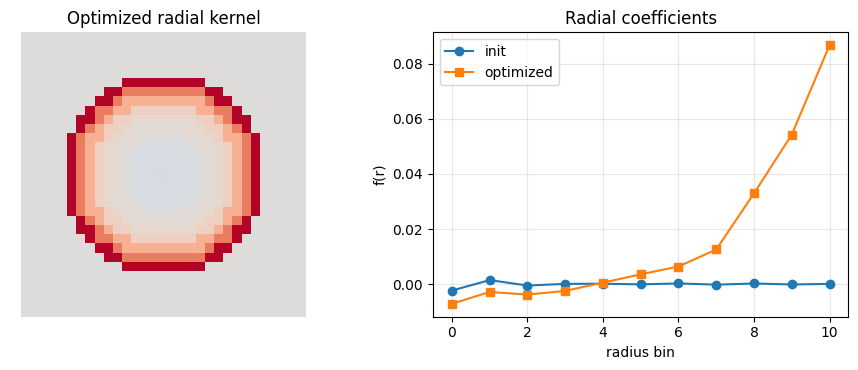
\includegraphics[width=0.49\linewidth]{figures/radial_fi_optimized_kernel_and_coefficients.png}
    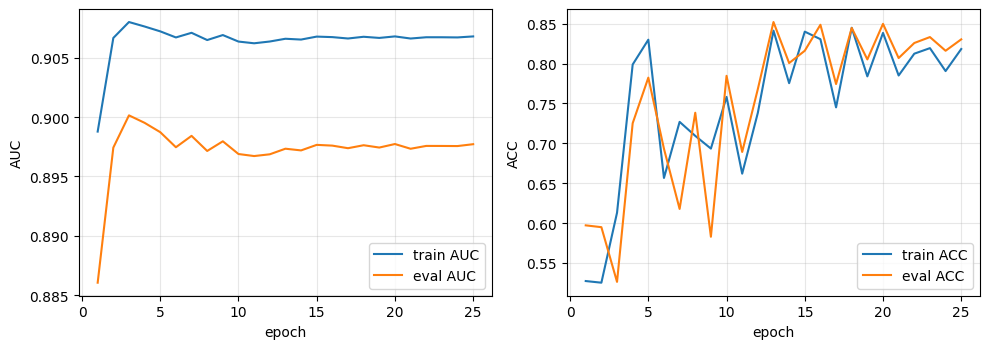
\includegraphics[width=0.49\linewidth]{figures/radial_kernel_fi_optimization_cell06_exec17_out02.png}
    \caption{Left: initial radial kernel, optimized radial kernel, and learned $f(r)$ coefficients. Right: training curves for train/eval AUC and ACC across epochs for the trained radial kernel ($f_i$ optimization).}
\end{figure}

\section*{Full-Image Inference + Heatmaps}
The figures below correspond to inference with the trained radial kernel (optimized via $f_i$ learning; kernel rotated every $10^\circ$). \\

\textbf{Set A (Invariant kernel, rotated every $10^\circ$):}
\begin{figure}[H]
    \centering
    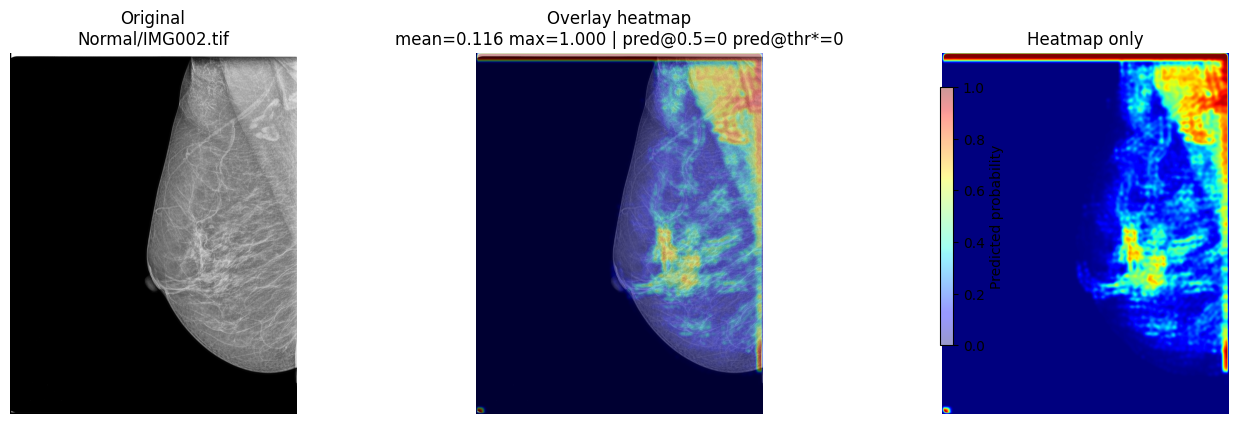
\includegraphics[width=0.49\linewidth]{figures/radial_kernel_fi_optimization_cell08_out02.png}
    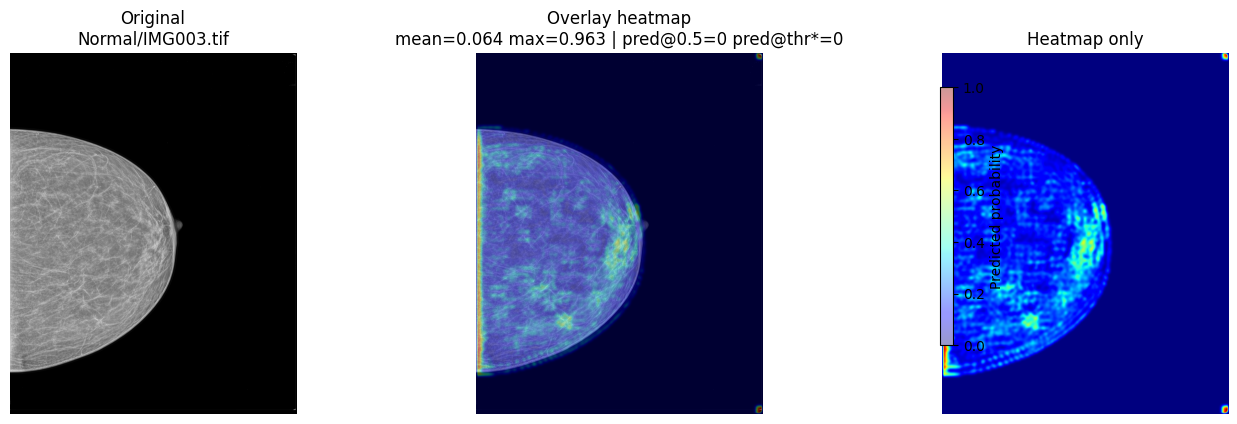
\includegraphics[width=0.49\linewidth]{figures/radial_kernel_fi_optimization_cell08_out03.png}
    \caption{Normal class, Set A examples 1--2 (trained radial kernel, rotated every $10^\circ$).}
\end{figure}

\begin{figure}[H]
    \centering
    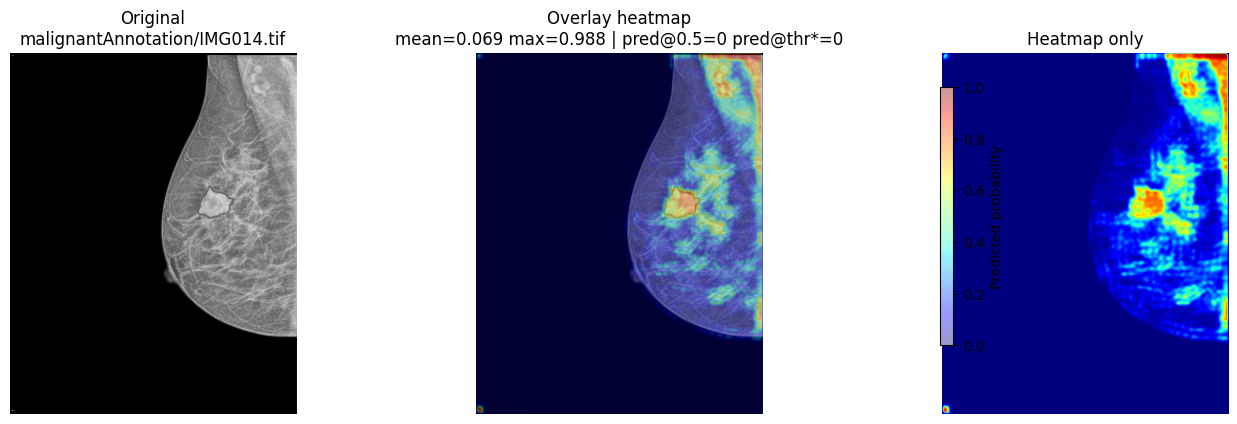
\includegraphics[width=0.49\linewidth]{figures/radial_kernel_fi_optimization_cell08_out06.png}
    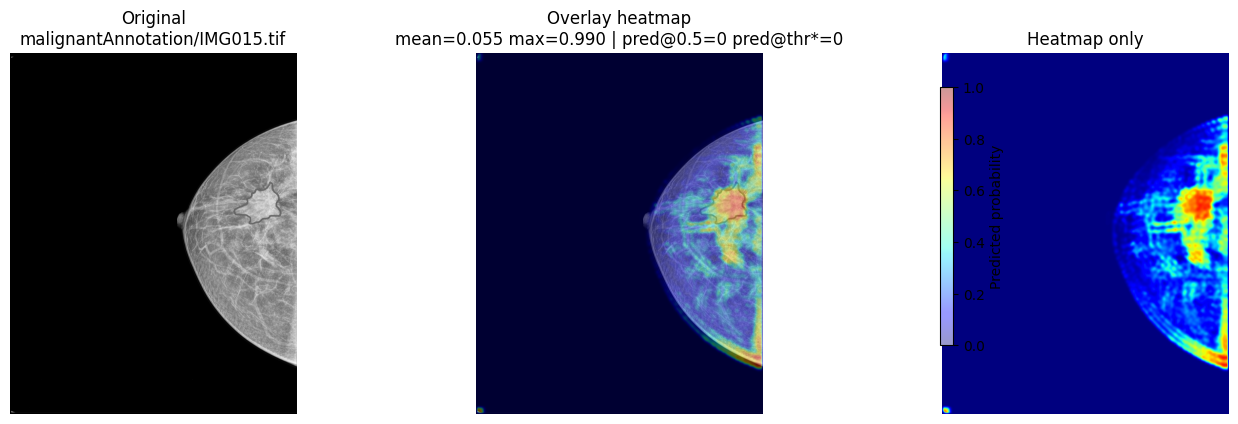
\includegraphics[width=0.49\linewidth]{figures/radial_kernel_fi_optimization_cell08_out07.png}
    \caption{malignant class, Set A examples 1--2 (trained radial kernel, rotated every $10^\circ$).}
\end{figure}

\textbf{Set B (Trained radial kernel):}
\begin{figure}[H]
    \centering
    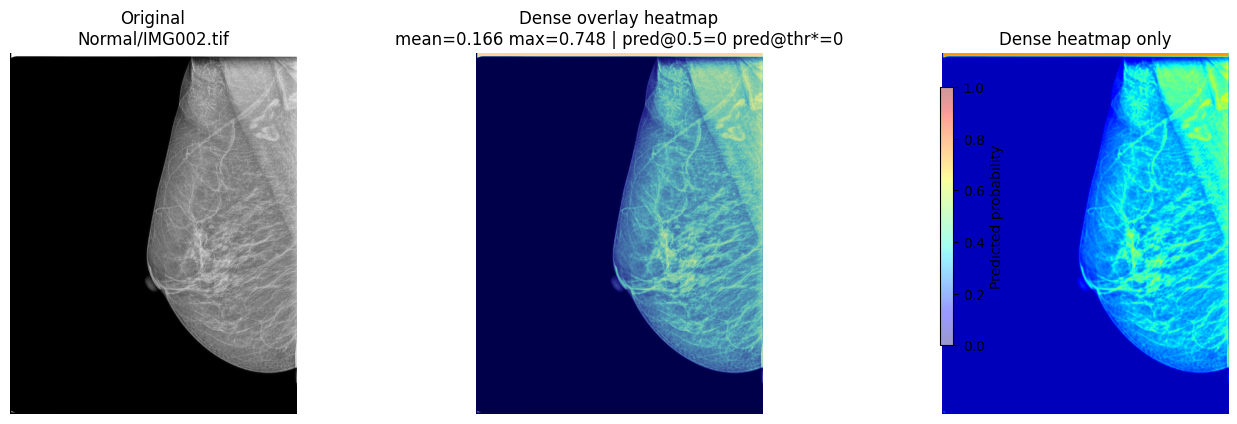
\includegraphics[width=0.49\linewidth]{figures/radial_kernel_fi_optimization_exec21_cell10_out02.png}
    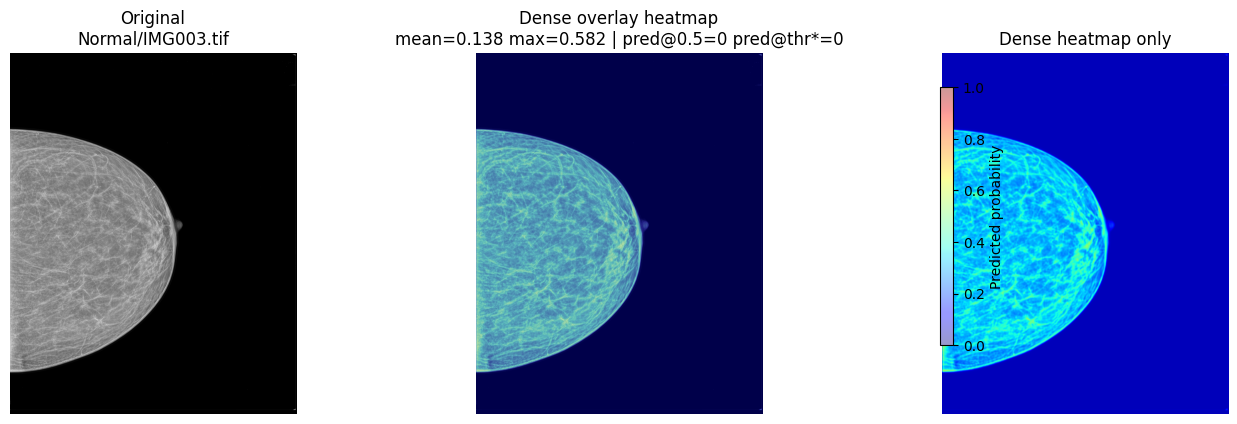
\includegraphics[width=0.49\linewidth]{figures/radial_kernel_fi_optimization_exec21_cell10_out03.png}
    \caption{Normal class, Set B examples 1--2 from trained-radial-kernel ($f_i$) inference.}
\end{figure}

\begin{figure}[H]
    \centering
    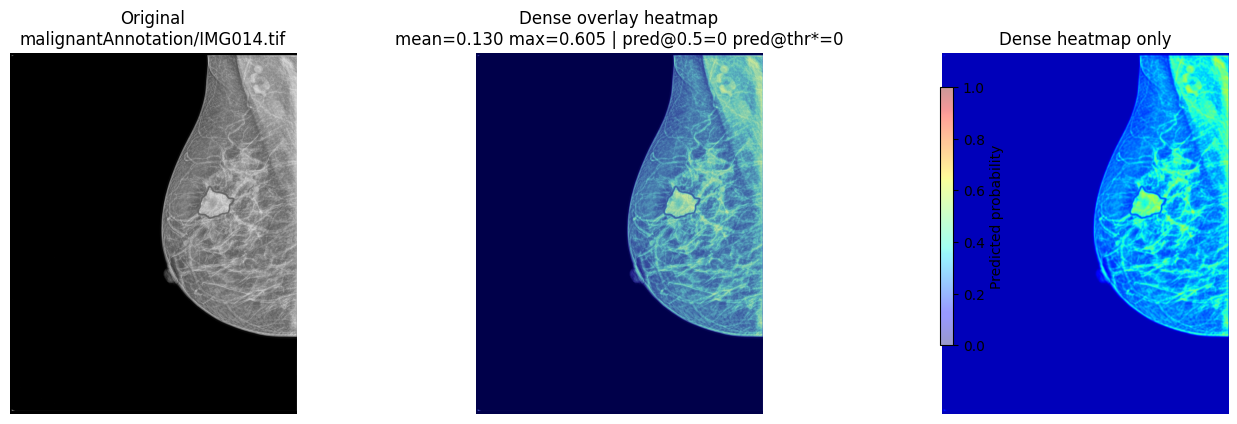
\includegraphics[width=0.49\linewidth]{figures/radial_kernel_fi_optimization_exec21_cell10_out06.png}
    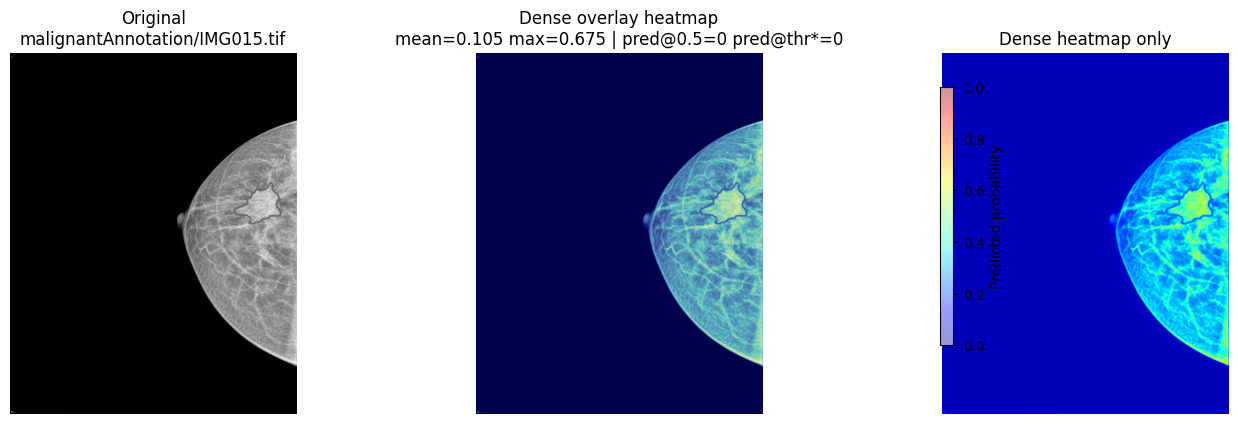
\includegraphics[width=0.49\linewidth]{figures/radial_kernel_fi_optimization_exec21_cell10_out07.png}
    \caption{malignant class, Set B examples 1--2 from trained-radial-kernel ($f_i$) inference.}
\end{figure}

\section*{Findings}
\begin{itemize}
    \item The radial-parameterized optimization of $f_i$ improved performance over the manually created invariant kernel baseline.
    \item Although the training metrics are very good, the heatmap quality does not perform well qualitatively.
\end{itemize}

\section*{Diagnosis}
Several refinements for heatmap behavior:
\begin{itemize}
    \item Reduced inference stride from coarse overlap to a finer setting.
    \item Added Gaussian patch-weight blending instead of uniform patch filling.
    \item Used smoother rendering (bilinear interpolation) and higher save DPI.
    \item Added a dense full-image inference block (per-pixel response map) to reduce square artifacts from patch-level aggregation.
\end{itemize}
These changes improved visual smoothness, but the qualitative localization is still weaker than expected in.

\section*{Next Steps}
\begin{itemize}
    \item Revisit the response definition for localization (e.g., avoid over-reliance on global max-like behavior).
    \item Use smaller patch size and/or multi-scale inference to improve spatial detail.
    \item Add hard-negative mining from normal images that still receive high heatmap scores.
    \item Evaluate localization with explicit region-level metrics (not only patch-level AUC/ACC).
\end{itemize}

\section*{Conclusion}
The trained radial-kernel approach with $f_i$ optimization gives strong quantitative performance in this run (best Eval AUC $=0.897333$, ACC@0.5 $=0.852000$), and it outperforms the invariant-kernel rotated-every-$10^\circ$ baseline (AUC $=0.875518$, ACC@0.5 $=0.793143$) while remaining stable across right-angle rotations. However, despite these good training/evaluation metrics, the qualitative full-image heatmaps are still not satisfactory. In summary, the method is promising for classification accuracy, but heatmap quality/localization needs further improvement before it can be considered reliable for visual interpretation.

\end{document}
